\documentclass[t]{beamer}
\usetheme{Madrid}
\usecolortheme{seahorse}
\definecolor{seahorse}{RGB}{189, 186, 238}
\setbeamercolor{block title}{bg=seahorse,fg=black}

\usepackage{multicol}
\usepackage{tikz}
\usepackage{amsmath}
\usepackage{amssymb}
\usepackage{tcolorbox}
\usepackage{mathtools}
\usepackage{mathrsfs}
\usepackage{physics}
\usepackage{enumitem}
\usepackage{bm}
\usepackage{bbm}

\title{Interaction between PDE and geometry}
\author[MAT264] 
{Kaja Jurak, Esther Jerez}

\institute[UIB]
{
  Faculty of Mathematics\\
  University of Bergen
  
}
\date[2021]
{May 2021}


\logo{
    \begin{tikzpicture}
        \node[inner sep=0pt] (logo) at (0,0)
            {
\includegraphics[width=.25\textwidth]{uiblogo.png}};
\end{tikzpicture}}


\setlength\parindent{0pt}
\begin{document}
    \frame{\titlepage}
    \begin{frame}
        \frametitle{Introduction}
        Our main goal is to give accurate error bounds for approximated solutions of a PDE. In concrete, we will focus on the problem of the steady-state heat equation, described by  \alert{Poison's equation}:
        \begin{align*}
            \bm{q} = -k \div ^2 u
        \end{align*}
    where 
    \begin{enumerate}
        \item[] $\bm{q}$ is the heat flux of the source,
        \item[] $k$ is the materials' thermal conductivity,
        \item[] $u$ is the temperature.
    \end{enumerate}
    With the previous PDE we will look at the flow rates or fluxes of energy locally. \\

        % \begin{block}{Remark}
        %     Sample text
        % \end{block}
    
    \end{frame}

    \begin{frame}
        \frametitle{Introduction}
        \begin{columns}[t]
            \column{0.5\textwidth}
            \textbf{1D CASE}
            \begin{align*}
                &\frac{\partial q}{\partial x} = f \\
                &q = -k \frac{\partial u}{\partial x} 
            \end{align*}
            And we will consider the following situations:
            \begin{itemize}
                \item[1.] Linear flux ($\frac{\partial q}{\partial x} = 1$) and constant thermal conductivity ($k=1$).
                \item[2.] Linear flux and thermal conductivity not constant.
                \item[3.] Flux non-linear ant thermal conductivity not constant.
            \end{itemize}
            
            \column{0.5\textwidth}
            \textbf{2D CASE} \\
            \begin{align*}
                &\frac{\partial q}{\partial x} + \frac{\partial q}{\partial y}  = f \\
                &\bm{q} = -k \left( \frac{\partial u}{\partial x} + \frac{\partial u}{\partial y}\right)
            \end{align*}
            But we will only consider a case where flux is linear ant the thermal conductivity is constant.
        \end{columns}        
    \end{frame}

    \begin{frame}
        \frametitle{Error bounds computations}
        We are considering a general elliptic PDE:
        \begin{align*}
            \div q = f , \quad q =-k \div u
        \end{align*}
        Main idea: instead of measuring $\norm*{u-v} = \norm*{e_v}$, study $\norm*{k^{\frac{1}{2}}\div e_v}$. 
        \\ By integrating the PDE and some more computations we obtain:
        \begin{align*}
            \norm*{k^{\frac{1}{2}}\div e:v} \leq \norm*{k^{-\frac{1}{2}}(\bm{r}+k\div v)} + C_{\Omega,k}\norm*{f-\div \bm{r}} \equiv \mathcal{M}(v,r;f)
        \end{align*}
        where $\bm{r}$ is an approximation to the flux function.
        With this error bound, we will also consider the \alert{relative error}:
        \begin{align*}
            \frac{\norm*{k^{\frac{1}{2}}\div e_v}}{\norm*{k^{\frac{1}{2}}\div v}} \leq \frac{\mathcal{M}(v,r;f)}{\norm*{k^{\frac{1}{2}}\div v}}
        \end{align*}
        
    \end{frame}

    \begin{frame}
        \frametitle{Error bounds computations}
        When we do know the the real solution, we will also compute the \alert{efficiency index} (for the potential):
        \begin{align*}
            I_v = \frac{\mathcal{M}(v,r;f)}{\norm*{k^{\frac{1}{2}}\div e_v}}
        \end{align*}
        Combine the energy errors of both the potential and the flux:
        \begin{align*}
            \norm*{(e_v,e_r)}_{*} \equiv \norm*{k^{\frac{1}{2}}\div e_v} + \norm*{k^{-\frac{1}{2}}e_r} + C_{\Omega,k}\norm*{\div e_r}
        \end{align*} 
        And indeed, we can prove with the previous concepts that 
        \begin{align*}
            \mathcal{M}(v,r;f) \leq  \norm*{(e_v,e_r)}_{*}  \leq 3\mathcal{M}(v,r;f)
        \end{align*}
    \end{frame}

    \begin{frame}
        \frametitle{Implementation of the method}
        \begin{multicols}{2}[\columnsep2em] 
                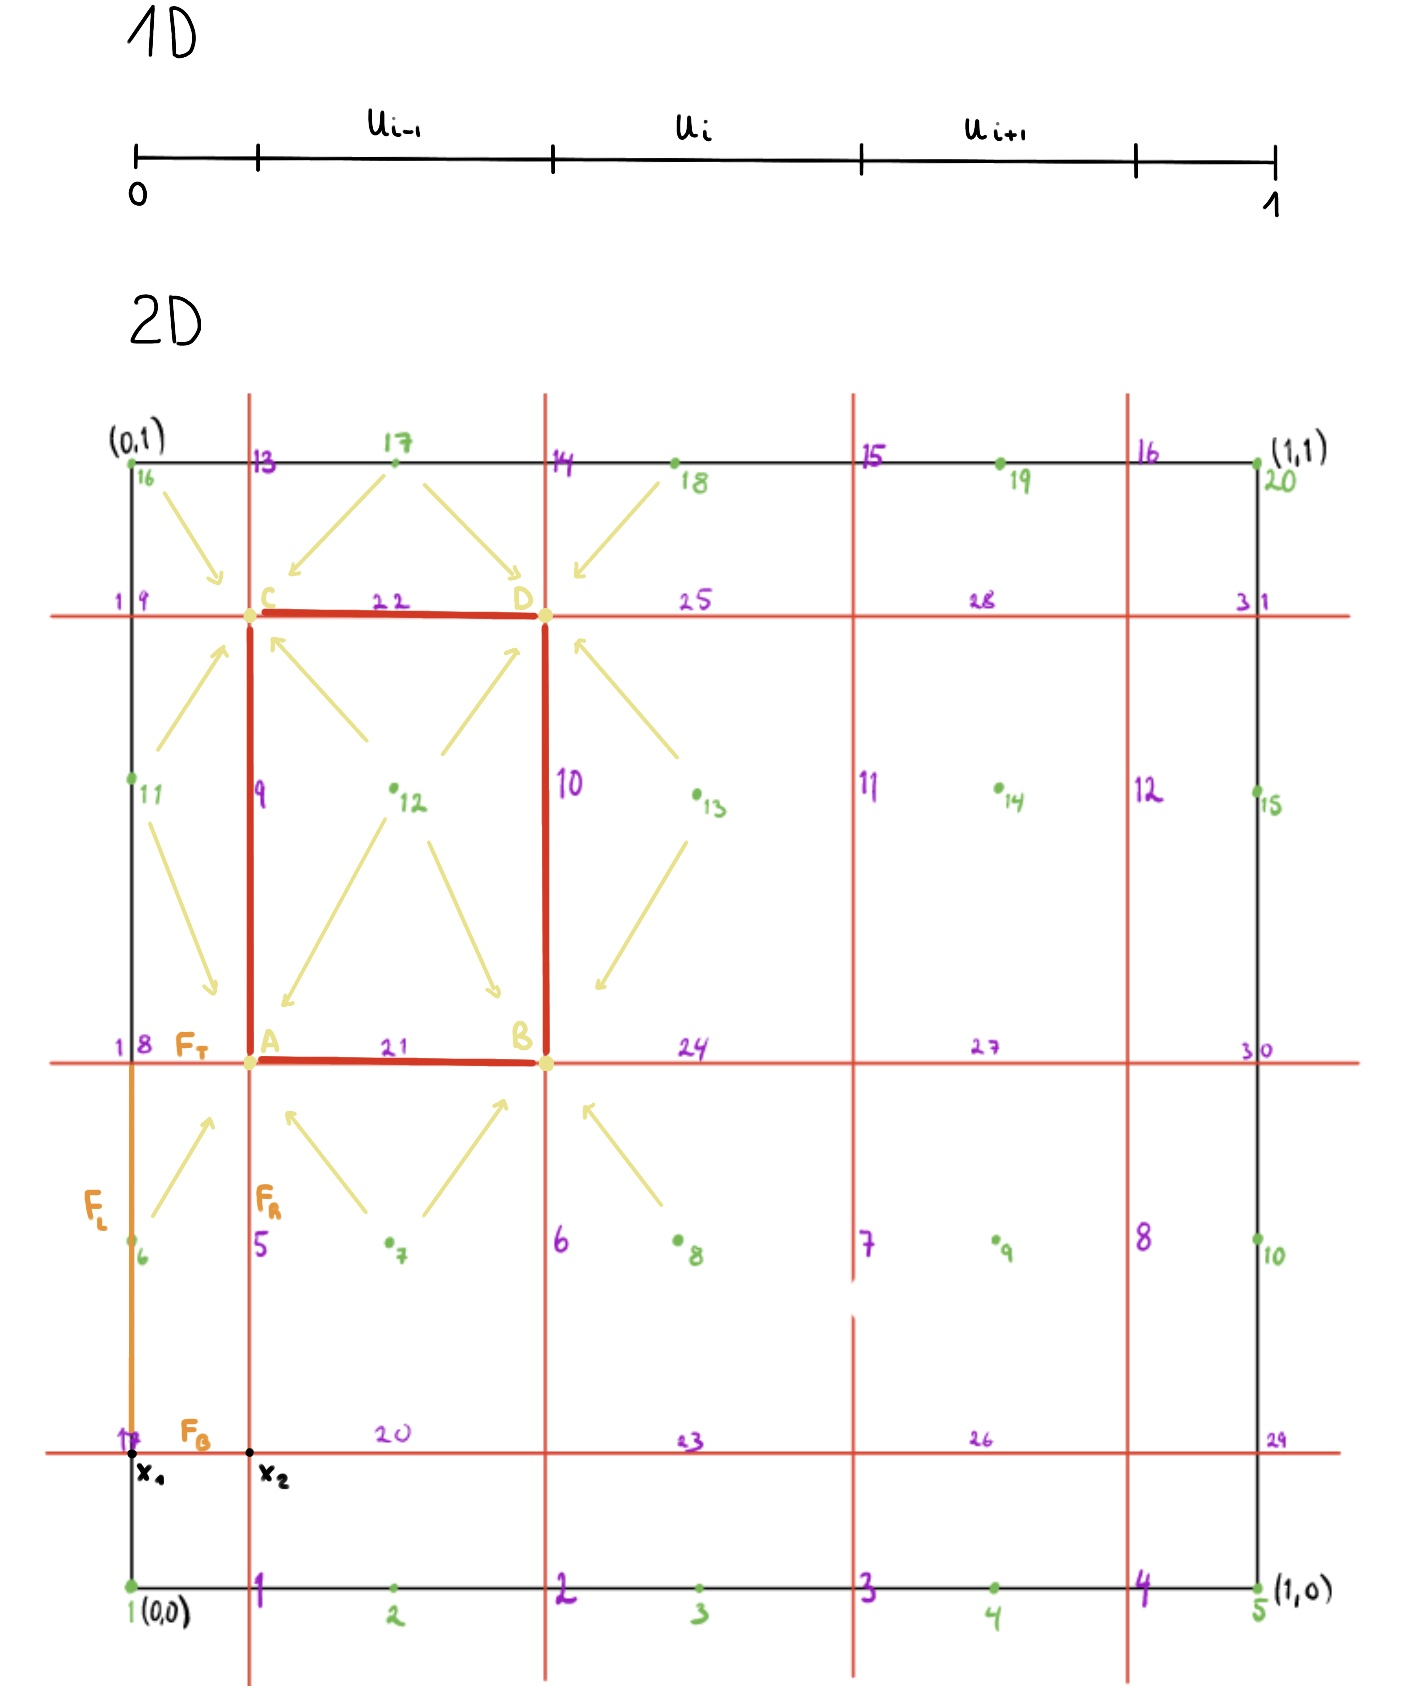
\includegraphics[width=\linewidth]{square.jpg}
                \columnbreak
                
                For each cell, we will approximate the potential ($v_h \approx u$), and the flux satisfies an integral form of conservation, so we can compute the flux ($r_h$) in every edge surrounding the cell using finite difference. Interpolating both flux and potential we can then obtain functions smooth enough to work with them. 
            \end{multicols}
                
    \end{frame}

    \begin{frame}
        \frametitle{Implementation of the method}
        
        If we are considering the 1D case, following the conservation law for cell $i$ we have:
        \begin{align*}
            q_{i+1} - q_i =  \int_{w_i} f
        \end{align*}

        This can be applied the same way in the 2D case, component by component. For the particular case of a left side cell we would compute the flux on the left edge by:
        \begin{align*}
            F_L &= F_R - \int\limits_{x_1}^{x_2} f(x,y) \,dx\ \\
            &=  F_R - f(x,y)\Delta x \quad \text{\scriptsize{(Cause we are considering f being constant)}}
        \end{align*}
    \end{frame}

    \begin{frame}
        \frametitle{Results in 1D}
    
    \end{frame}

    \begin{frame}
        \frametitle{Results in 2D}
    
    \end{frame}

    \begin{frame}
        \frametitle{Conclusion}
    
    \end{frame}

    \begin{frame}
        \frametitle{References}
    
    \end{frame}
\end{document}
    